\section{Density Conclusions}


 The density experiment provided an excellent opportunity to validate the relationship between Coho density/biomass and eDNA accumulation. Using a Coho specific DNA primer, we were able to detect Coho at all levels of density, ranging from 1 fish to 65 fish. To model mean TCT of Coho eDNA, we chose models that contained biomass as a predictor. The impact of tank appeared to be due to human error in the cleaning of the tanks. Overall, we confirmed that Coho biomass is highly correlated with an increase in mean TCT. We fit both median and mean TCT, and it would be up to a researcher to decide which they prefer to work with. Robust models provided very similar estimates compared to their linear model counterparts and we thus chose to continue only with linear models.



\begin{table}[H]
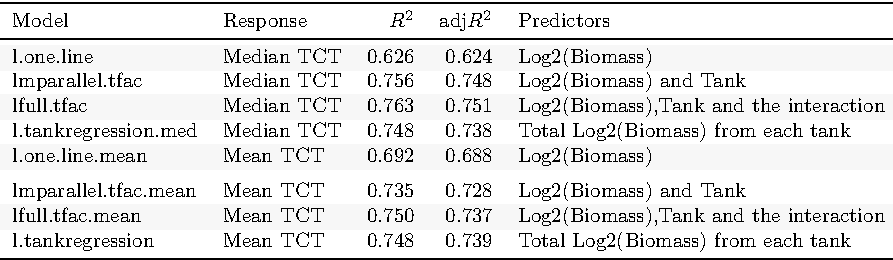
\includegraphics{Chapter3Images/densitymodelsummary.pdf}
\caption{Summary table for the linear models we created. We include the Response, the $R^{2}$ and the adjusted $R^{2}$.}
\label{fig:modelsummary}
\end{table}
\vspace{5mm}

One highlight of our analysis was the creation of Figure~\ref{fig:medct55}, which summarizes much of the results of the experiment in one concise image. Collapsing by taking the mean TCT value over each tank proved to be useful and provided a simple model, l.tankregression. This model performed well, evidenced by the high adjusted $R^{2}$ ( Table~\ref{fig:modelsummary}) and the distribution of the model residuals (Figure~\ref{lab:resid22}). 

\vspace{5mm}

In the density experiment, Coho eDNA was detected with 100\%  certainty at all densities ranging from 1 to 65 fish per tank. In regard to detection of technical replicates, perfect detection was achieved at all densities from 4 to 65 fish. For 2 fish, one technical replicate failed to detect Coho. For 1 fish, only three sample replicates indicated non-detection. We thus were also able to validate the performance and high levels of sensitivity of the eONKI4 DNA assay in the detection of Coho Salmon. A small pilot experiment also was used to gain insight regarding the background signal of Coho in the hatchery water. As seen in Figure~\ref{lab:introplots1232} and Figure~\ref{lab:introplots123222}, the hatchery water contained a small but non-consistent amount of evidence of Coho eDNA.




